\subsection{Data}

\subsubsection{Training Data}
All files published to Tableau Public through February 2014 were scanned. We collected the contents of columns with names containing any of the following strings: Date, month, created, dt (abbreviation for date), mes (month in Spanish), datum (date in German), fecha (date in Spanish), data (date in Portuguese), ? (day in Chinese and Japanese). Roughly 95\% of the data in Tableau Public is in English, but we attempted to include non-English data that was available. Fields of any data type other than date or datetime were analyzed, including strings, integers, and floats. One file was created for each scanned column, containing the unique non-null values in the column.

The resulting set of files were de-duplicated. This handles any duplicate files on Tableau Public including sample data. Files over 1MB were manually reviewed and those that did not contain dates removed. There were 30,968 files in the resulting set.
Most database and spreadsheet systems already detect a limited set of date formats. For instance, typing the string \texttt{"12/31/1999"} into Microsoft Excel, is automatically interpreted as the date \texttt{1999-12-31}. The Microsoft Jet library that Tableau used to read these text files detects a few date formats as well. Any column already converted by Excel or Jet was not included in this study.

\textbf{Verification Data}\\
Verification used another set of data from Tableau Public, collected through April 2015. This set was collected similarly, but also added columns named time. We limited this set to new Tableau Excel and text connectors that were released in May 2014. It is likely that some of these files were older files republished to Tableau Public. There were 31,546 files in the resulting set.

The new Tableau text connector is able to automatically interpret a somewhat different limited set of date formats. Any column already converted by Excel or the new Tableau text connector was not included in this study.

\subsection{Evaluation}
Once the training data was analyzed, it was grouped by date format. A sample of each produced date format was manually labeled. This allowed us to quickly skip over very common formats like \texttt{MM/dd/yyyy} and focus our efforts on much less common formats. The samples were judged as to whether the produced format was reasonable and were tagged with correct formats if the produced format was unreasonable.

Further manual tagging focused on the files most likely to represent dates. Many of the files in the collection are not actually dates, such as fields named ``updated by'' (which contain ``date''). A random sample of 850 columns named exactly ``date", ``time'' or ``month'' (case-insensitive) were manually judged.

\subsubsection{	Minimum Descriptive Length}
Testing of the MDL algorithm was performed on a 24-core Dell T7610 running Windows 7 with the data stored on a 250GB SSD.


\begin{table}[ht]
\begin{tabular}{|p{0.48\linewidth}| p{0.48\linewidth}|}
\hline
\textbf{Number of Records} & 31,546\\ \hline
\textbf{Error Rate} & 27.95\% \\ \hline
\textbf{Analysis Speed ($\mu s$)} & 2,245.04 \\ \hline
\textbf{Validation Speed ($\mu s$)} & 1.65 \\ \hline
\textbf{Median Not Null} & 50 \\ \hline
\end{tabular}
\label{tab:mdlstats}
\caption{MDL Parsing Statistics.}
\end{table}



To test the MDL algorithm, we ran it over the set of samples from each validation file to generate a ranked list of formats for the file. Each format was then applied to the entire file�s data set, recording both the number of errors and the elapsed times. In cases where we generated multiple formats and the main format produced errors, we applied the second format to the unparsed strings. The summary statistics from this processing are presented in Table 2.

The analysis speed is the average time needed per sample for structure extraction. At 2.5ms, this is well below most human perceptual thresholds for a set of 32 samples, so any latency in command execution would be restricted to the ability of the underlying database to provide the samples for analysis in a timely manner. (As a column store, the TDE can often supply such domains without a full table scan, further improving responsiveness.) 

The validation speed is the average time needed to parse a value, and provides an estimate of how fast an ICU-based implementation (such as the TDE) can process string values into scalars and works out to 620K values per core per second.
 
\begin{figure}[ht]
\centering
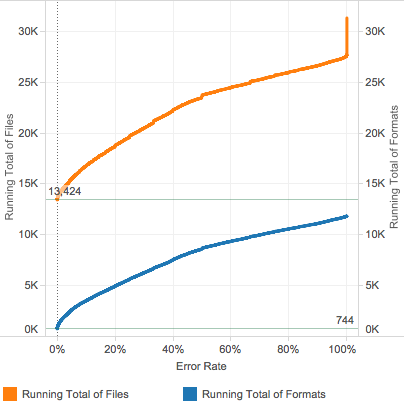
\includegraphics[width=\columnwidth]{figures/FigureM2}
\caption{MDL Error Rate}
\label{fig:M2}
\end{figure}


The error rate reflects the fact that only about 40\% of the files have an associated format that parses the non-null values without error. To examine the error rate in greater detail, we turn now to Figure \ref{fig:M2}.

On the left hand side, we can see that the algorithm found 744 distinct formats that parsed 13,424 files with no error. This is a remarkable number of valid formats and underscores the need for this kind of algorithm. Raising the error rate threshold to 5\% results in about 2500 formats found in 15,000 files, or nearly half of the files. 

What do these formats look like? Figure \ref{fig:M3} shows a histogram of the 25 most common formats containing a year format code at the 5\% threshold, color-coded by error rate. (A sample value is provided to the right of each bar for illustrative purposes.) The formats have also been filtered to files with at least 5 samples. Most of the samples are clearly dates with a wide range of formats (the format where the time zone is between the time and the year is surprisingly common.)
 
\begin{figure}[ht]
\centering
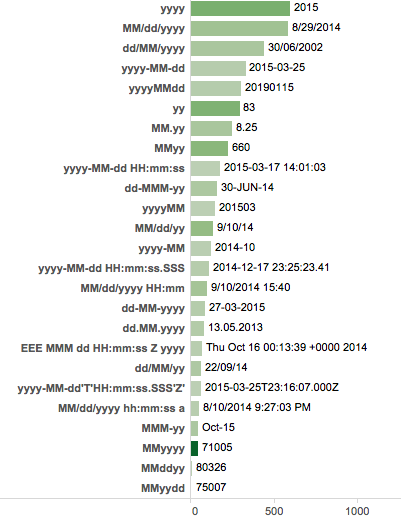
\includegraphics[width=\columnwidth]{figures/FigureM3}
\caption{MDL Output}
\label{fig:M3}
\end{figure}


Some of the dates are clearly just numbers, but our approach is to assume that when the user tells us that the column contains dates we should find the best fit. The samples include dates from a wide range of historical sources (e.g. Roman pottery dates) so we have elected to defer the date identification task to the user.

\subsubsection{Natural Language Processing}

\subsubsection{	Cross-Checking}
